\documentclass{beamer}
%\documentclass[trans]{beamer}

\usetheme[%pageofpages=/,% String used between the current page and the total page count.
%bullet=circle,% Use circles instead of squares for bullets.
titleline=true,% Show a line below the frame title.
alternativetitlepage=true,% Use the fancy title page.
%titlepagelogo=logo-polito,% Logo for the first page.
]{Torino} 

\newcommand{\code}[1]{\textbf{#1}}

\usepackage{parcolumns}
\usepackage{listings} 
\usepackage{subfig}
\author{Lasse Folger}
\title{\huge Alternative Software Transactional Memory Implementation in Haskell}
\subtitle{Master Thesis}
\date{05.04.2017}

\lstset{escapeinside=!!}
\begin{document}
  \begin{frame}[t,plain]
    \titlepage
  \end{frame}
  
  
  \begin{frame}
    \frametitle{Motivation}
    \lstinputlisting{ressources/accountMVar.hs}
  \end{frame}
  
  \begin{frame}[fragile]
    \frametitle{MVar}
    \fboxsep=0pt
    \noindent
    \begin{minipage}[t]{0.48\linewidth}
      Thread 1:
            \begin{figure}
       \begin{lstlisting}[frame=single]
transfer acc1 acc2 50
       \end{lstlisting}
      \end{figure}
\end{minipage}%
    \hfill%
    \begin{minipage}[t]{0.48\linewidth}
      Thread 2:      
      \begin{figure}
       \begin{lstlisting}[frame=single]
transfer acc2 acc1 50
       \end{lstlisting}
      \end{figure}
    \end{minipage}
\end{frame}

  \begin{frame}[fragile]
    \frametitle{MVar}
    \fboxsep=0pt
    \noindent
    \begin{minipage}[t]{0.48\linewidth}
      Thread 1:
            \begin{figure}
       \begin{lstlisting}[frame=single]
a1 <- takeMVar acc1 
a2 <- takeMVar acc2 
writeMVar acc1 (a1 - 50)
writeMVar acc2 (a2 + 50)
       \end{lstlisting}
      \end{figure}
\end{minipage}%
    \hfill%
    \begin{minipage}[t]{0.48\linewidth}
      Thread 2:      
      \begin{figure}
       \begin{lstlisting}[frame=single]
b1 <- takeMVar acc2 
b2 <- takeMVar acc1 
writeMVar acc2 (b1 - 50)
writeMVar acc1 (b2 + 50)
       \end{lstlisting}
      \end{figure}
    \end{minipage}
    \vfill
    \pause
    $\Rightarrow$ Deadlock
\end{frame}
  
  \begin{frame}
    \frametitle{Use Transactions}
    \lstinputlisting{ressources/accountTVar.hs}   
  \end{frame}
  
  \begin{frame}[fragile]
    \frametitle{TVar}
    \fboxsep=0pt
    \noindent
    \begin{minipage}[t]{0.48\linewidth}
      Thread 1:
      \begin{figure}
       \begin{lstlisting}[frame=single]
atomically $ 
  transfer acc1 acc2 50
       \end{lstlisting}
      \end{figure}
    \end{minipage}%
    \hfill%
    \begin{minipage}[t]{0.48\linewidth}
      Thread 2:
      \begin{figure}
       \begin{lstlisting}[frame=single]
atomically $ 
  transfer acc2 acc1 50
       \end{lstlisting}
      \end{figure}
    \end{minipage}
    \vfill
    \pause
    $\Rightarrow$ works fine, because transactions provide ACI(D) properties
\end{frame}
%%%%%%%%%%%%%%%%%%%%%%%%%%%%
%%%Current Implementation%%%
%%%%%%%%%%%%%%%%%%%%%%%%%%%%
  \begin{frame}
    \frametitle{Current Implementation (Control.Concurrent.STM)}
    \begin{itemize}\setlength\itemsep{1em}
      \item \textit{writeTVar}, \textit{readTVar} and \textit{newTVar} modify TVars
      \item \textit{retry} and \textit{orElse} alter the control flow
      \item \textit{atomically} executes a transaction 
      \item composition via bind operator (or do)
    \end{itemize}
  \end{frame}
  
  \begin{frame}
   \frametitle{Transactional Log}
   \begin{itemize}\setlength\itemsep{1em}
    \item one log per transaction
    \item necessary for consistency
    \item three elements per log entry
          \begin{itemize}
           \item \code{TVar}
           \item \code{expectedValue}
           \item \code{currentValue}
          \end{itemize}
   \end{itemize}
  \end{frame}
  
  \begin{frame}
   \frametitle{Modify Operations}
   \begin{itemize}\setlength\itemsep{1em}
    \item \textbf{newTVar}: creates a new, initialized TVar 
    \item \textbf{writeTVar}: updates \textit{currentValue} in log entry
    \item \textbf{readTVar}: reads TVar from log or actual TVar
  \end{itemize}
\end{frame}
  
\begin{frame}[fragile]
\frametitle{Example}
\begin{lstlisting} 
transaction = do
  a <- readTVar t1
  writeTVar t2 a
  readTVar t2
\end{lstlisting}
\vfill
\pause
Log after first action:
\begin{lstlisting}
 [(t1,a,a)]
\end{lstlisting}
\end{frame}
  
\begin{frame}[fragile]
\frametitle{Example}
\begin{lstlisting} 
transaction = do
  a <- readTVar t1
  writeTVar t2 a
  readTVar t2
\end{lstlisting}
\vfill
Log after second action:
\begin{lstlisting}
 [(t1,a,a), (t2,b,a)]
\end{lstlisting}
\end{frame}


\begin{frame}[fragile]
\frametitle{Example}
\begin{lstlisting} 
transaction = do
  a <- readTVar t1
  writeTVar t2 a
  readTVar t2
\end{lstlisting}
\vfill
Log after thrid action:
\begin{lstlisting}
 [(t1,a,a), (t2,b,a)]
\end{lstlisting}
\end{frame}
     
  \begin{frame}
   \frametitle{\lstinline{atomically :: STM a -> IO a}}
   \begin{enumerate}\setlength\itemsep{1em}
    \item compute the log
    \item lock TVars
    \item validate the log
    \item if valid then commit
    \item else roll back
   \end{enumerate}
  \end{frame}

  \begin{frame}
   \frametitle{Validation}
    \begin{enumerate}\setlength\itemsep{1em}
      \item compare \textit{expectedValue} to the value in the actual TVar
      \item if all values match return valid 
      \item else return invalid
    \end{enumerate}
  \end{frame}

%%%%%%%%%%%%%%%%%% 
%%%%%Problems%%%%%
%%%%%%%%%%%%%%%%%%

\begin{frame}[fragile]
    \frametitle{Problem}
    \fboxsep=0pt
    \noindent
    \begin{minipage}[t]{0.48\linewidth}
      Thread 1:
    \begin{figure}
     \begin{lstlisting}[frame=single]
a1 <- readTVar acc1
a2 <- readTVar acc2
writeTVar acc1 (a1 - 50)
writeTVar acc2 (a2 + 50)
     \end{lstlisting}
    \end{figure}
    Log:
    \begin{figure}
     \begin{lstlisting}[frame=single]
[(acc1, a1, a1-50),
 (acc2, a2, a2+50)]
     \end{lstlisting}
    \end{figure}
    \end{minipage}%
    \hfill%
    \begin{minipage}[t]{0.48\linewidth}
      Thread 2:
    \begin{figure}
     \begin{lstlisting}[frame=single]
b1 <- readTVar acc2
b2 <- readTVar acc1
writeTVar acc2 (b1 - 50)
writeTVar acc1 (b2 + 50)
     \end{lstlisting}
    \end{figure}
Log:
    \begin{figure}
     \begin{lstlisting}[frame=single]
[(acc2, b1, b1-50),
 (acc1, b2, b2+50)]
    \end{lstlisting}
    \end{figure}
    \end{minipage}
\end{frame}

\begin{frame}[fragile]
    \frametitle{Problem}
    \fboxsep=0pt
    \noindent
    \begin{minipage}[t]{0.48\linewidth}
      Thread 1:
    \begin{figure}
     \begin{lstlisting}[frame=single]
[(acc1, a1, a1-50),
 (acc2, a2, a2+50)]
     \end{lstlisting}
    \end{figure}
    \end{minipage}%
    \hfill%
    \begin{minipage}[t]{0.48\linewidth}
      Thread 2:
    \begin{figure}
     \begin{lstlisting}[frame=single]
[(acc2, b1, b1-50),
 (acc1, b2, b2+50)]
     \end{lstlisting}
    \end{figure}
    \end{minipage}
    \vfill
    \pause
    $\Rightarrow$ either sequential or one transaction is rolled back
\end{frame}


\begin{frame}
 \frametitle{Critical TVar}
   \begin{itemize}\setlength\itemsep{1em}
    \item critical between read and commit
    \item modifications to critical TVars cause rollback
   \end{itemize}
   \pause
   \vfill
   $\Rightarrow$ minimize the time TVars are critical 
\end{frame}


  
  \begin{frame}
   \frametitle{Critical TVar}
   \begin{figure}
    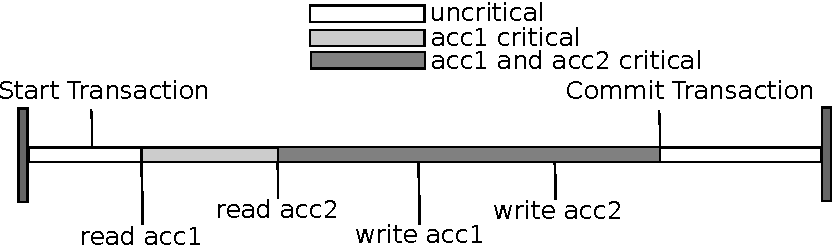
\includegraphics[scale=0.7]{ressources/CriticalValue.pdf}
   \end{figure}
   \end{frame}

\begin{frame}[fragile]
\frametitle{Idea}
\begin{lstlisting}
transfer = do 
  a1 <- readTVar acc2
  writeTVar acc2 (a1 - 50)
  a2 <- readTVar acc1
  writeTVar acc1 (a2 + 50)
\end{lstlisting}
\end{frame}
  
     
  \begin{frame}
   \frametitle{Critical TVar}
   \begin{figure}
    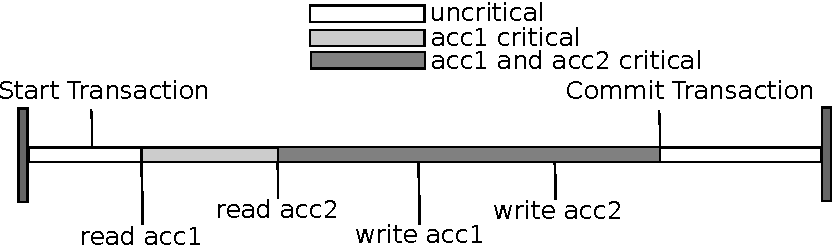
\includegraphics[scale=0.7]{ressources/CriticalValue.pdf}
   \end{figure}
   \begin{figure}
    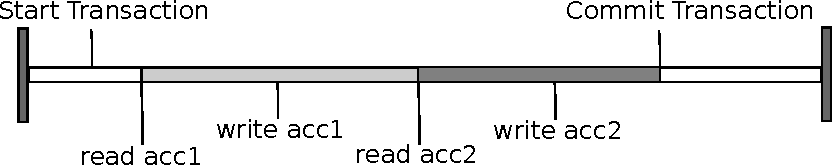
\includegraphics[scale=0.7]{ressources/CriticalValue2.pdf}
   \end{figure}
   \end{frame}

\begin{frame}
 \frametitle{Idea}
 \begin{itemize}\setlength\itemsep{1em}
  \item delay the evaluation of \code{readTVar} to commit phase
  \item no TVars is critical at all  
  \item \code{writeTVar} does not need the value in the computation phase
 \end{itemize}
\end{frame}
  
\begin{frame}[fragile]
   \frametitle{Idea does not work}
   \begin{lstlisting}[language=Haskell]
limitedTransfer src dst am = do
   a1 <- readTVar src
   if a1 < am
     then return ()
     else do a2 <- readTVar dst
             writeTVar src (a1 - am)
             writeTVar dst (a2 + am)
   \end{lstlisting}
   \vfill
   $\Rightarrow$ idea does not work because the value is needed.
\end{frame}

%%%%%%%%%%%%%%%%%
%%%%%Concept%%%%%
%%%%%%%%%%%%%%%%%

  \begin{frame}
   \frametitle{Solution}
   \begin{itemize}\setlength\itemsep{1em}
    \item delay evaluation as far as possible
    \item evaluate reads just before they are needed..
    \item ..or in the commit phase
   \end{itemize}
  \end{frame}


  \begin{frame}
   \frametitle{When is a value needed?}
   \begin{itemize}\setlength\itemsep{1em}
    \item branch conditions
       \begin{itemize}
        \item if-then-else
        \item case
        \item patternmatching
        \item guards
       \end{itemize}
    \item IO-actions $\Rightarrow$ not allowed in STM
   \end{itemize}
  \end{frame}
  
  \begin{frame}
    \frametitle{Example}
    \lstinputlisting{ressources/accountTVar.hs}   
  \end{frame}
  
  \begin{frame}[fragile]
   \frametitle{Example: limitedTransfer acc1 acc2 5}
   \begin{lstlisting}[language=Haskell]
a1 <- readTVar acc1
if a1 < 5
  then return ()
  else do a2 <- readTVar acc2
          writeTVar acc1 (a1 - am)
          writeTVar acc2 (a2 + am)
   \end{lstlisting}
   \pause
   \begin{figure}
    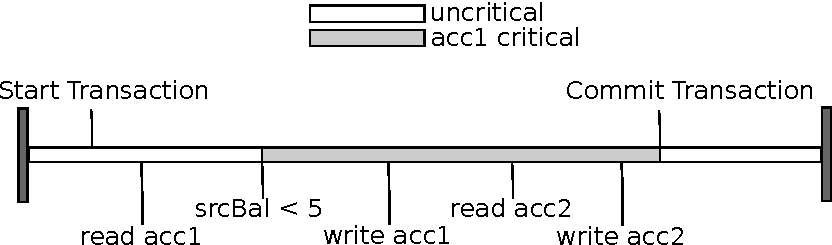
\includegraphics[scale=0.7]{ressources/lessCriticalValue.pdf}
   \end{figure}
\end{frame}
  
%%%%%%%%%%%%%%%%%%%%%%%%%%%
%%%%%My Implementation%%%%%
%%%%%%%%%%%%%%%%%%%%%%%%%%%

  \begin{frame}
  \frametitle{Implementation}
  \begin{itemize}\setlength\itemsep{1em}
   \item pure Haskell implementation
   \item state monad
   \item computation phase modifies the state 
   \item commit phase uses state to validate and commit
  \end{itemize}
  \end{frame}

  \begin{frame}
  \frametitle{State}
  \begin{itemize}\setlength\itemsep{1em}
   \item read log
   \item write log
   \item unevaluated reads
  \end{itemize}
  \end{frame}

  
  \begin{frame}
  \frametitle{writeTVar}
  \begin{itemize}\setlength\itemsep{1em}
   \item search TVar in write log
   \item \code{readTVar} creates an read expression and extends write log
   \item \code{unsafePerformIO} :: IO a $\rightarrow$ a 
   \item IO action logs the information in read log
  \end{itemize}
  \end{frame}

  \begin{frame}
  \frametitle{Computation Phase}
  \begin{itemize}\setlength\itemsep{1em}
   \item \code{writeTVar} modifies write log
   \item \code{newTVar} does not access the state
   \item computation phase is evaluation of the STM action 
  \end{itemize}
  \end{frame}

  
  \begin{frame}
  \frametitle{Commit Phase}
  \begin{enumerate}\setlength\itemsep{1em}
   \item lock TVars in write log
   \item validate read log
   \item evaluate remaining reads
   \item publish modifications
  \end{enumerate}
  \end{frame}
  
  
%%%%%%%%%%%%%%%%%%%%
%%%%%Evaluation%%%%%
%%%%%%%%%%%%%%%%%%%%

  \begin{frame}
  \frametitle{Evaluation}
  \begin{itemize}\setlength\itemsep{1em}
   \item STM is universal tool
   \item unlimited possibilities
   \item testing is challenging
  \end{itemize}
  \end{frame}

  \begin{frame}
  \frametitle{Evaluation}
  \begin{itemize}\setlength\itemsep{1em}
   \item tested specific cases
   \item increase in level of concurrency
   \item results meet the expectations
  \end{itemize}
  \end{frame}
   
\begin{frame}
\begin{figure}
\centering
 \begin{tabular}[center]{|c|c|c|c|}
  \hline
	                       & GHC    & Project & STMLA  \\ \hline
  medium concurrency  & 3.0420 &  3.2830 & 2.9225 \\ \hline
  low concurrency     & 3.0670 &  3.3110 & 2.9425 \\ \hline
  high concurrency    & 3.1520 &  3.4335 & 2.9455 \\ \hline
 \end{tabular}
\end{figure}
\end{frame}
  
  
%%%%%%%%%%%%%%%%%%%%%
%%%%%Future Work%%%%%
%%%%%%%%%%%%%%%%%%%%%
 
\begin{frame}[fragile]
\frametitle{Future Work: True Consistency}
\begin{lstlisting}
transaction = do 
  a <- readTVar t1
  b <- readTVar t2
  if b == a 
    then return ()
    else loop
\end{lstlisting}
\end{frame} 
 
 \begin{frame}
  \frametitle{Future Work: Exception Handling}
   \begin{itemize}\setlength\itemsep{1em}
    \item exception handling
    \item validate before passing an exception
    \item if invalid roll back
    \item unlock TVars when expection occurs
   \end{itemize}
  \end{frame}
  
\begin{frame}
 \frametitle{Future Work}
 \begin{itemize}\setlength\itemsep{1em}
  \item invariants 
  \item C library with compiler integration
  \item further performance testing
 \end{itemize}
\end{frame}

 

\begin{frame}
 \frametitle{Questions about...}
 \begin{itemize}\setlength\itemsep{1em}
  \item ...Control.Concurrent.STM?
  \item ...rollback avoidance?
  \item ...my implementation?
  \item ...something else?
\end{itemize}
\end{frame}


  
\end{document}



